\documentclass{standalone}
\usepackage{tikz}
\begin{document}
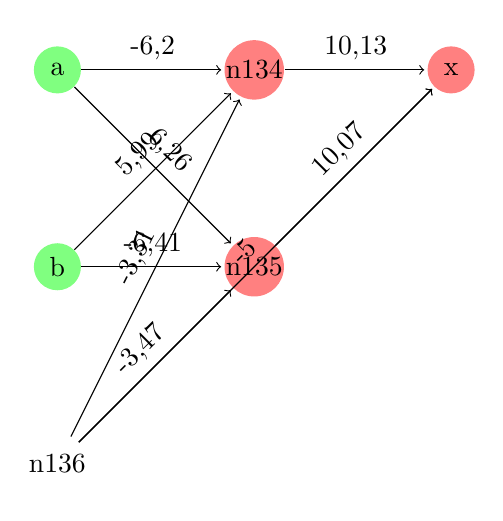
\begin{tikzpicture}[shorten >=1pt,->,draw=black!,node distance=2.5cm]
\tikzstyle{neuron}=[circle,fill=black!25,minimum size=17pt,inner sep=0pt]
\tikzstyle{constant}=[neuron, fill=white!50];
\tikzstyle{identity}=[neuron, fill=green!50];
\tikzstyle{sigmoid}=[neuron, fill=red!50];
\node [identity] (a) {a};
\node [identity,below of=a] (b) {b};
\node [constant,below of=b] (n136) {n136};
\node [sigmoid,right of=a] (n134) {n134};
\node [sigmoid,below of=n134] (n135) {n135};
\node [sigmoid,right of=n134] (x) {x};
\path[every node/.style={sloped,anchor=south,auto=false}]
(a) edge node {6,26} (n135)
(a) edge node {-6,2} (n134)
(b) edge node {5,99} (n134)
(b) edge node {-6,41} (n135)
(n136) edge node {-5} (x)
(n136) edge node {-3,31} (n134)
(n136) edge node {-3,47} (n135)
(n134) edge node {10,13} (x)
(n135) edge node {10,07} (x)
;\end{tikzpicture}
\end{document}